\documentclass{../project}

\usepackage{xcolor}
\usepackage{physics}
\usepackage{amsmath}
\usepackage{tikz}
\usepackage{mathdots}
\usepackage{yhmath}
\usepackage{cancel}
\usepackage{color}
\usepackage{siunitx}
\usepackage{array}
\usepackage{multirow}
\usepackage{amssymb}
\usepackage{gensymb}
\usepackage{tabularx}
\usepackage{extarrows}
\usepackage{booktabs}
\usepackage{wrapfig}
\usetikzlibrary{fadings}
\usetikzlibrary{patterns}
\usetikzlibrary{shadows.blur}
\usetikzlibrary{shapes}

\begin{document}

\begin{sheet}[title={Project 4: Partial differential equations (PDEs)}, number=4, due={December 20th, 10am}]

\begin{problem}[title={Laplace equation}, label=laplace]

\begin{wrapfigure}{r}{4.0cm}
  %\caption{A wrapped figure going nicely inside the text.}\label{wrap-fig:1}
    \tikzset{every picture/.style={line width=0.75pt}} %set default line width to 0.75pt        

    \begin{center}
    \vspace{-1.5cm}

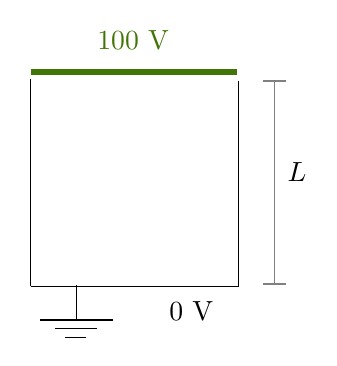
\begin{tikzpicture}[x=0.75pt,y=0.75pt,yscale=-1,xscale=1]
%uncomment if require: \path (0,300); %set diagram left start at 0, and has height of 300

%Straight Lines [id:da052861809245647984] 
\draw    (50.5,40) -- (50.5,140) ;
%Straight Lines [id:da6911112292195916] 
\draw    (150.67,41) -- (150.67,140) ;
%Straight Lines [id:da4793716242372551] 
\draw    (50.5,140) -- (150.67,140) ;
%Straight Lines [id:da12601847792163] 
\draw [color={rgb, 255:red, 65; green, 117; blue, 5 }  ,draw opacity=1 ][line width=2.25]    (50.5,37) -- (150,37) ;
%Straight Lines [id:da3433856794707031] 
\draw    (72.67,139.67) -- (72.67,156.33) ;
%Straight Lines [id:da17376056318444277] 
\draw    (90.33,156.33) -- (55,156.33) ;
%Straight Lines [id:da12786273869981946] 
\draw    (82.33,160.33) -- (62.33,160.33) ;
%Straight Lines [id:da609271959418566] 
\draw    (77,164.67) -- (67,164.67) ;
%Straight Lines [id:da32675694375407927] 
\draw [color={rgb, 255:red, 128; green, 128; blue, 128 }  ,draw opacity=1 ]   (168,41) -- (168,139) ;
\draw [shift={(168,139)}, rotate = 270] [color={rgb, 255:red, 128; green, 128; blue, 128 }  ,draw opacity=1 ][line width=0.75]    (0,5.59) -- (0,-5.59)   ;
\draw [shift={(168,41)}, rotate = 270] [color={rgb, 255:red, 128; green, 128; blue, 128 }  ,draw opacity=1 ][line width=0.75]    (0,5.59) -- (0,-5.59)   ;

% Text Node
\draw (81.33,15.73) node [anchor=north west][inner sep=0.75pt]  [color={rgb, 255:red, 65; green, 117; blue, 5 }  ,opacity=1 ]  {$100\ \text{V}$};
% Text Node
\draw (116,146.4) node [anchor=north west][inner sep=0.75pt]    {$0\ \text{V}$};
% Text Node
\draw (173,79.4) node [anchor=north west][inner sep=0.75pt]    {$L$};
\end{tikzpicture}

    \end{center}
\end{wrapfigure} 

  Consider the two-dimensional setup of a square box
  with a side length of $L$, where the top edge
  is set to a potential of \SI{100}{\volt}
  and the other three edges are grounded, i.e.\ at a potential of zero.
  Your task is to find the potential within the box,
  where it solves the Laplace equation
  \begin{equation}
    \Delta \phi(x,y) = 0.
  \end{equation}

  \begin{subproblem}[label=laplace:a,points=6]
    Write a program that computes the potential $\phi(x,y)$
    within the box with a discretisation length of $\Delta x = L/100$.
    Implement the Jacobi, Gauß--Seidel and SOR methods.
    As a stopping criterion, assert that the error
    of the discretised Laplace equation
    is smaller than $\epsilon_\text{max}=10^{-3}\,\text{V}$ everywhere.
    The error is defined as
    $\epsilon_{i,j} = |\phi_{i,j} - (\phi_{i+1,j} + \phi_{i-1,j} + \phi_{i,j+1} + \phi_{i,j-1})/4|$.
    Plot the average and maximum error versus the number of iterations
    for all algorithms.
    For SOR, use four different over-relaxation parameter values $\alpha=0.5, 1.0, 1.25, 1.5, 1.75$ and $1.99$.
    Check if it still converges for $\alpha \geq 2.0$.
    Discuss your results.
  \end{subproblem}

  \begin{subproblem}[label=laplace:c,points=4]
    The solution of this problem can be written
    as an infinite series:
    \begin{equation}
      \phi(x,y) = \sum_{n=1,3,5,\ldots}^{\infty}
      \frac{400}{n\pi}
      \sin\left(\frac{n \pi y}{L}\right)
      \exp(-n \pi x).
      %\frac{
      %  \sinh(n \pi y / L)
      %}{
      %  \sinh(n \pi)
      %}
    \end{equation}
    Plot this solution for 1, 10, 100 and 1000 terms.
    Plot the difference between one of the iterative solutions
    and the ``infinite'' series solution using 1000 terms.
    %Compare the computing time needed in both cases.
    Discuss your results.
  \end{subproblem}

  \iffalse

  Now let's move on to a parallel-plate capacitor inside a grounded box
  \textcolor{red}{Make figure}.
  We will consider three variants of this setup.

  \begin{subproblem}[label=laplace:d,points=4]
    For the simplest version,
    assume that the plates are very thin
    and the top one is maintained at $\SI{100}{\volt}$
    and the bottom one at $\SI{-100}{\volt}$.
    Use SOR to find the solution of $\phi(x,y)$,
    then plot it and discuss your result.
    Discuss your choice of the spatial discretisation
    and the convergence of the SOR algorithm.
  \end{subproblem}

  \begin{subproblem}[label=laplace:e,points=4]
    Now assume that the plates have a finite thickness
    of two $\Delta$s,
    and that they have a uniform charge density of
    $\rho$ at the top plate and 
    $-\rho$ at the bottom one.
    Solve Poisson's equation for the points inside the plates
    and Laplace's equation everywhere else using SOR.
    Experiment until you find a value for $\rho$ that gives
    a similar potential to that found in \ref{laplace:d},
    and report that value.
  \end{subproblem}

  \begin{subproblem}[label=laplace:f,points=4]
    Now keep the finite thickness used in \ref{laplace:e},
    but use fixed voltages of $\pm\SI{100}{\volt}$ again.
    Solve Laplace's equation to find $\phi(x,y)$ in the volume
    outside of the plates (and within the box).
    Then use Poisson's equation
    to calculate the charge density within the plates.
    Plot your solution for $\phi(x,y)$ (everywhere) and for $\rho$ (within the plates).
    What can you observe?
  \end{subproblem}

  \fi

\end{problem}

\clearpage
\begin{problem}[title={Diffusion}, label=diffusion]

% Pattern Info
 
\tikzset{
pattern size/.store in=\mcSize, 
pattern size = 5pt,
pattern thickness/.store in=\mcThickness, 
pattern thickness = 0.3pt,
pattern radius/.store in=\mcRadius, 
pattern radius = 1pt}
\makeatletter
\pgfutil@ifundefined{pgf@pattern@name@_kaet050nx}{
\pgfdeclarepatternformonly[\mcThickness,\mcSize]{_kaet050nx}
{\pgfqpoint{0pt}{0pt}}
{\pgfpoint{\mcSize+\mcThickness}{\mcSize+\mcThickness}}
{\pgfpoint{\mcSize}{\mcSize}}
{
\pgfsetcolor{\tikz@pattern@color}
\pgfsetlinewidth{\mcThickness}
\pgfpathmoveto{\pgfqpoint{0pt}{0pt}}
\pgfpathlineto{\pgfpoint{\mcSize+\mcThickness}{\mcSize+\mcThickness}}
\pgfusepath{stroke}
}}
\makeatother

% Gradient Info
  
\tikzset {_aqpbluvlt/.code = {\pgfsetadditionalshadetransform{ \pgftransformshift{\pgfpoint{0 bp } { 0 bp }  }  \pgftransformrotate{0 }  \pgftransformscale{2 }  }}}
\pgfdeclarehorizontalshading{_f47b4jjoh}{150bp}{rgb(0bp)=(0.8,1,0.96);
rgb(37.5bp)=(0.8,1,0.96);
rgb(50bp)=(0.96,0.65,0.14);
rgb(62.5bp)=(0.8,1,0.96);
rgb(100bp)=(0.8,1,0.96)}
\tikzset{every picture/.style={line width=0.75pt}} %set default line width to 0.75pt        

  Consider a metallic rod of a finite length $L$ and a small radius,
  which is isolated at its side,
  but not at its ends, where it is placed in contact
  with ice water at $\SI{0}{\celsius}$:
    \begin{center}
\begin{tikzpicture}[x=0.75pt,y=0.75pt,yscale=-1,xscale=1]
%uncomment if require: \path (0,300); %set diagram left start at 0, and has height of 300

%Shape: Rectangle [id:dp5864415645155785] 
\draw  [fill={rgb, 255:red, 205; green, 255; blue, 244 }  ,fill opacity=1 ] (58.5,103) -- (310.5,103) -- (310.5,189) -- (58.5,189) -- cycle ;
%Rounded Rect [id:dp897577066365276] 
\draw  [fill={rgb, 255:red, 155; green, 155; blue, 155 }  ,fill opacity=1 ] (100,135) .. controls (100,130.58) and (103.58,127) .. (108,127) -- (258.5,127) .. controls (262.92,127) and (266.5,130.58) .. (266.5,135) -- (266.5,159) .. controls (266.5,163.42) and (262.92,167) .. (258.5,167) -- (108,167) .. controls (103.58,167) and (100,163.42) .. (100,159) -- cycle ;
%Rounded Rect [id:dp7154176973964292] 
\draw  [pattern=_kaet050nx,pattern size=6pt,pattern thickness=0.75pt,pattern radius=0pt, pattern color={rgb, 255:red, 0; green, 0; blue, 0}] (100,135) .. controls (100,130.58) and (103.58,127) .. (108,127) -- (258.5,127) .. controls (262.92,127) and (266.5,130.58) .. (266.5,135) -- (266.5,159) .. controls (266.5,163.42) and (262.92,167) .. (258.5,167) -- (108,167) .. controls (103.58,167) and (100,163.42) .. (100,159) -- cycle ;
%Shape: Rectangle [id:dp3634772346802485] 
\path  [shading=_f47b4jjoh,_aqpbluvlt] (93,142) -- (273.5,142) -- (273.5,152) -- (93,152) -- cycle ; % for fading 
 \draw  [line width=1.5]  (93,142) -- (273.5,142) -- (273.5,152) -- (93,152) -- cycle ; % for border 

%Curve Lines [id:da3957444069652777] 
\draw    (264.5,77) .. controls (303.3,75.06) and (295.06,86.29) .. (277.18,112.52) ;
\draw [shift={(275.5,115)}, rotate = 304.16] [fill={rgb, 255:red, 0; green, 0; blue, 0 }  ][line width=0.08]  [draw opacity=0] (8.93,-4.29) -- (0,0) -- (8.93,4.29) -- cycle    ;
%Curve Lines [id:da9902844569020139] 
\draw    (127.5,216) .. controls (150.54,216.96) and (144.09,193.96) .. (135.57,171.77) ;
\draw [shift={(134.5,169)}, rotate = 68.63] [fill={rgb, 255:red, 0; green, 0; blue, 0 }  ][line width=0.08]  [draw opacity=0] (8.93,-4.29) -- (0,0) -- (8.93,4.29) -- cycle    ;
%Curve Lines [id:da4643989745761563] 
\draw    (255.5,211) .. controls (278.54,211.96) and (282.23,179.74) .. (274.52,156.81) ;
\draw [shift={(273.5,154)}, rotate = 68.63] [fill={rgb, 255:red, 0; green, 0; blue, 0 }  ][line width=0.08]  [draw opacity=0] (8.93,-4.29) -- (0,0) -- (8.93,4.29) -- cycle    ;

% Text Node
\draw (120.5,67.4) node [anchor=north west][inner sep=0.75pt]    {$\text{Ice water at } T\ =\ 0\degree $};
% Text Node
\draw (65,207) node [anchor=north west][inner sep=0.75pt]   [align=left] {Isolation};
% Text Node
\draw (188,202) node [anchor=north west][inner sep=0.75pt]   [align=left] {Metal rod};


\end{tikzpicture}
    \end{center}
  To simulate the temperature flow,
  we will need to solve the diffusion PDE
  \begin{equation}
    \pdv{T(x,t)}{t} = \frac{K}{C \rho} \frac{\partial^2 T(x,t)}{\partial x^2},
  \end{equation}
  with the thermal conductivity $K$, the heat capacity $C$ and the density $\rho$.
  Use $L=1$, $K=210$, $C=900$ and $\rho = 2700$, and, if not otherwise specified,
  $\Delta x = 0.01$ and $\Delta t = 0.1$ with a number of time steps $N_t = 10000$.
  The rod's temperature distribution
  is initially set to $T(x,0)=\sin(\pi x/L)$.

  \begin{subproblem}[label=laplace:a,points=8]
    Simulate the system using the FTCS algorithm and plot $T(x, t)$.
  \end{subproblem}
  \begin{subproblem}[label=laplace:b,points=4]
    The analytical solution is given by
    \begin{equation}
      T_\text{exact}(x,t) = \sin\left(\frac{\pi x}{L}\right) \exp\left(-\frac{\pi^2 K t}{L^2 C \rho}\right).
    \end{equation}
    With that, we can define our simulation error as
    \begin{equation}
      \epsilon(t) = \frac{1}{N_x} \sum_{j=1}^{N_x-1}|T(j\Delta x,t) - T_\text{exact}(j\Delta x,t)|,
    \end{equation}
    where $N_x = L / \Delta x$.
    Study the behaviour of $\epsilon(t=100)$
    varying $\Delta t$ between $0.001$ and $0.7$
    while keeping $\Delta x$ fixed.
    What happens? Explain your finding.
  \end{subproblem}
  \begin{subproblem}[label=laplace:c,points=4]
    Now, implement the implicit Euler backward, the Crank--Nicolson and Dufort--Frankel algorithms
    and repeat the analysis for $\epsilon(t=100)$ for all of them.
    Discuss your results comparing the four algorithms,
    in particular with respect to the scaling behaviour
    of the error with $\Delta t$.
  \end{subproblem}

  \iffalse
  \begin{subproblem}[label=laplace:b,points=4]
    In the following, the rod initially has a homogeneous temperature of $T_0=\SI{100}{\celsius}$.
    Plot a 3D plot with the axes $x$, $t$ and $T(x, t)$.
    Discuss your solution.
  \end{subproblem}
  \fi

\end{problem}

\clearpage
\begin{problem}[title={Solitons}, label=solitons]


  Water waves
  in shallow, narrow channels
  can be described by the Koorteweg--de Vries (KdeV) equation
  \begin{equation}
    \pdv{u(x,t)}{t}
    + \epsilon u(x,t) \pdv{u(x,t)}{x}
    + \mu \frac{\partial^3 u(x,t)}{\partial x^3} = 0.
  \end{equation}
  The non-linear term leads to a sharpening of the wave
  and ultimately to a shock wave.
  In contrast, the $\partial^3 u / \partial x^3$ term
  produces broadening.
  For the proper parameters and initial conditions,
  the two effects exactly balance each other,
  and a stable wave is formed,
  which is called a ``soliton''.
  These stable solitons almost behave as particles,
  and appear in many areas of physics.
  For more details on the numerical discovery of this fascinating phenomenon, see
  ``\href{https://physics.aps.org/articles/v6/15}{Computer Simulations Led to Discovery of Solitons}''.
  For a deeper dive, you can also download the original paper from
  \href{https://www.studip.uni-goettingen.de/dispatch.php/course/files/index/456b3abe95c2a22ac980707f6d7e1368?cid=1a9a322e21be361e60889361d2ce1a0f}{Stud.IP \goto\ Übung: Methods of Computational Physics \goto\ Files \goto\ Additional Material}.

  Inserting the traveling wave ansatz $u(x,t) = u(x-ct)$
  gives a solvable ODE with the (non-trivial) solution
  \begin{equation}
    u(x,t)=\frac{-c}{2} \sech^2\left( \frac{1}{2} \sqrt c (\xi - \xi_0) \right),
  \end{equation}
  where $\xi = x - ct$ is the phase.
  Note that the amplitude is proportional to the propagation speed $c$.
  Discretising the KdeV equation gives the algorithm
  \begin{align}
    \begin{split}\label{eq:kdev}
    u^{n+1}_j
    \approx
    u^{n-1}_j
      &- \frac{\epsilon}{3} \frac{\Delta t}{\Delta x} \left[ u_{j+1}^{n} + u_{j}^{n} + u_{j-1}^{n} \right]
      \left[u_{j+1}^{n} - u_{j-1}^{n}\right] \\
    &\quad- \mu \frac{\Delta t}{\Delta x^3}
      \left[ u_{j+2}^{n} + 2u_{j-1}^{n} - 2u_{j+1}^{n} - u_{j-2}^{n} \right].
    \end{split}
  \end{align}
  To calculate $u_{j}^{2}$, the first term on the right-hand side is not yet available,
  so we use a simpler forward difference scheme for the time step, which gives
  \begin{align}
    \begin{split}\label{eq:kdev_step1}
      u_{j}^{2}
    \approx
      u_{j}^{1}
      &- \frac{\epsilon}{6} \frac{\Delta t}{\Delta x} \left[ u_{j+1}^{1} + u_{j}^{1} + u_{j-1}^{1} \right]
      \left[u_{j+1}^{1} - u_{j-1}^{1}\right] \\
    &\quad- \frac\mu2 \frac{\Delta t}{\Delta x^3}
      \left[ u_{j+2}^{1} + 2u_{j-1}^{1} - 2u_{j+1}^{1} - u_{j-2}^{1} \right].
    \end{split}
  \end{align}
  In addition to the first time step, we also need to treat
  $u_{1}^n$, $u_{2}^n$, $u_{N_\text{max}-1}^n$ and $u_{N_\text{max}}^n$
  separately,
  since also they can not be updated using Eq.~\eqref{eq:kdev}.
  Given the initial state we will use below,
  a simple method is to use the constant boundary values $u_{1}^n=1$ and $u_{N_\text{max}}^n=0$.
  This leaves
  $u_{2}^n$ and $u_{N_\text{max}-1}^n$.
  These are still to be calculated using Eqs.~\eqref{eq:kdev} and~\eqref{eq:kdev_step1},
  but with the replacements
  $u_{0}^n \to u_{1}^n$ (when calculating $u_{2}^n$)
  and
  $u_{N_\text{max}+1}^n \to u_{N_\text{max}}^n$ (when calculating $u_{N_\text{max}-1}^n$)
  on the right-hand sides.

  \begin{subproblem}[label=solitons:a,points=4]
    Derive Eq.~\eqref{eq:kdev}. For the first derivates, use the central difference approximations
    $\partial u / \partial t \approx (u_j^{n+1} - u_j^{n-1})/(2\Delta t)$
    and
    $\partial u / \partial x \approx (u_{j+1}^n - u_{j-1}^n)/(2\Delta x)$.
    To find an approximation for the third derivative
    expand $u(x,t)$ to including $\mathcal O(\Delta x^4)$
    about the four points
    $u(x\pm \Delta x, t)$
    and
    $u(x\pm 2\Delta x, t)$,
    then solve for $\partial^3 u / \partial x^3$.
    Finally, for the non-differentiated $u(x,t)$
    in the second term of Eq.~\eqref{eq:kdev},
    use the average over three adjacent points,
    i.e.\ $u = (u_{j-1}^n + u_{j}^n + u_{j+1}^n)/3$.
    In your derivation, keep track of the
    truncation error, to prove that Eq.~\eqref{eq:kdev}
    is of order $\mathcal O(\Delta t^3) + \mathcal O(\Delta t \Delta x^2)$.
  \end{subproblem}

  \begin{subproblem}[label=solitons:b,points=8]
    Implement the above algorithm solving the KdeV equation
    for the initial condition
    \begin{equation}
      u(x,t=0) = \frac12 \left[ 1 - \tanh\left(\frac{x-25}{5}\right)\right].
    \end{equation}
    The parameters are given by $\epsilon = 0.2$ and $\mu=0.1$
    and the step sizes by $\Delta x = 0.4$ and $\Delta t = 0.1$.
    Use 130 steps in $x$, such that our simulation volume
    is given by $L=130\Delta x = 52$.
    Verify that these constants satisfy the stability condition
    \begin{equation}
      \frac{\Delta t}{\Delta x} \left[ \epsilon |u| + 4 \frac{\mu}{(\Delta x)^2}\right] \leq 1.
    \end{equation}
    Store the solution every 250 or so time steps
    and run the simulation for about 2000 time steps.
    Plot the disturbance $u$ versus position and versus time.
    Scott Russell observed in 1834
    in the Edinburgh-Glasgow canal that an initial, arbitrary wave form
    set in motion evolves into two or more solitary waves that move at different velocities.
    Can you confirm his observation?
    Into how many solitary waves does your initial wave form break up into?
  \end{subproblem}

  \begin{subproblem}[label=solitons:c,points=4]
    Explore what happens when a tall soliton collides with a short one.
    Do they bounce off each other? Do they go through each other?
    Do they interfere?
    Do they destroy each other?
    Does the tall soliton still move faster than the short one after collision?
    Start off by placing a tall soliton of height 0.8 at $x=12$,
    and a small soliton in front of it at $x=26$:
    \begin{equation}
      u(x,t=0) = 0.8 \left[ 1 - \tanh^2\left(\frac{3x}{12}-3\right)\right]
               + 0.3 \left[ 1 - \tanh^2\left(\frac{4.5x}{26}-4.5\right)\right].
    \end{equation}
    Make sure to adapt the constant boundary values for $u_1^n$ and $u_{N_\mathrm{max}}^n$
    for this simulation.
  \end{subproblem}

\end{problem}

\end{sheet}

\end{document}
